% intro_interprete.tex -- fragment LaTeX (sans préambule).
% Révision de style du 24 oct. 2026 : texte resserré ; faits, chiffres, citations, renvois et notes conservés.
\section{Un interprète français dans l'armée britannique}

Au 25~juillet 1916, premier jour du carnet, Hippolyte Combes, simple soldat non combattant, est depuis plus d'un an interprète à la Mission militaire française attachée à l'armée britannique. Il vit avec une compagnie hippomobile du train de la 18\textsuperscript{th}~(Eastern) Division, puis, à partir de novembre 1916, avec un service d'achat de paille et de foin de la Fifth Army. Le carnet ne raconte pas la bataille, mais l'arrière-front britannique, vu par un intermédiaire entre une armée étrangère et la population française.

\subsection{La Mission militaire française et ses interprètes}

En août 1914, plus de cinq cents interprètes français attendaient le corps expéditionnaire britannique dans les ports de débarquement. Sous-officiers réservistes pour la plupart, souvent choisis pour avoir vécu en pays de langue anglaise, ils assuraient la liaison avec les unités françaises voisines et surtout les rapports avec la population : cantonnement, réquisitions, dommages. Ils étaient environ trois mille en 1917\footnote{J.~Beach et J.~Bruce, «~Improvising Language Capability: The British Army's Corps of Interpreters, 1914--1915~», \textit{War in History}, 2023 (DOI 10.1177/09683445221140305), manuscrit accepté, p.~3--4 ; préface de François de Tessan à Fernand-Laurent, \textit{Chez nos alliés britanniques. Notes et souvenirs d'un interprète}, Paris, Boivin, 1917, p.~\textsc{xiii} : «~De cinq cents au début, ils sont devenus trois mille environ~».}. Ils relevaient de la Mission, dirigée par le général Victor Huguet puis, à partir de la fin de 1915, par le général Pierre des Vallières, officier de liaison au grand quartier général de Haig\footnote{E.~Greenhalgh (éd.), \textit{Liaison: General Pierre des Vallières at British General Headquarters, January 1916 to May 1917}, Army Records Society, vol.~36, 2016. Archives de la Mission : Service historique de la Défense, GR~17~N, cartons 295--486 (447--486 : listes nominatives, fiches individuelles et carnets de notes des interprètes) ; J.~Nicot, Ph.~Schillinger et J.~Ficat, \textit{Inventaire sommaire des archives de la guerre 1914--1918}, Vincennes, Service historique de l'Armée, 1972, p.~259--269. Ces dossiers n'ont pas été consultés.}.

Pendant la guerre, on y entrait par un «~examen d'interprète~», dont «~la première épreuve consistait en une conversation anglaise~»\footnote{Préface de F.~de Tessan, \textit{op.~cit.}, p.~\textsc{viii}.}. Les universitaires y étaient «~pourtant en majorité~», écrit Hippolyte Combes en février 1916, à propos d'un sous-officier interprète qui traitait les professeurs de «~rudes ânes~»\footnote{Copie autographe d'une lettre d'Hippolyte Combes à un capitaine, «~ancien camarade à la Faculté de Toulouse~», datée «~Au front, le 25~février 1916~», archives familiales (voir l'annexe, doc.~1).}. En 1917, l'Association des professeurs de langues vivantes demanda que les deux tiers des interprètes soient pris parmi les universitaires ; l'autorité militaire refusa le pourcentage, mais promit de tenir compte des diplômes\footnote{Allocution du président de l'Association à l'assemblée générale du 13~décembre 1917, \textit{Les Langues modernes}, 16\textsuperscript{e}~année, 1918, p.~5--6.}. Parmi les collègues d'Hippolyte Combes, le carnet nomme un professeur au lycée de Toulon (f.~48~v\textsuperscript{o}) et un professeur de Pont-à-Mousson (f.~65~r\textsuperscript{o}).

La hiérarchie avait trois degrés : les officiers interprètes, en trois classes, du sous-lieutenant au capitaine ; les interprètes stagiaires, au rang d'adjudant ; les interprètes auxiliaires, ou de complément, hommes de toutes armes, du soldat à l'adjudant, qui gardaient les insignes de leur corps et portaient en plus un sphinx de métal sur un écusson bleu\footnote{A.~F.~Whittem et P.~W.~Long, \textit{French for Soldiers}, Cambridge (Mass.), Harvard University Press, 1917, p.~130.}. Partis en 1914 dans l'uniforme de leur arme, les interprètes passèrent ensuite au kaki, avec képi ou casque (fig.~\ref{fig:interprete}) et, au collet, une tête de sphinx, souvenir des interprètes de l'expédition d'Égypte\footnote{Préface de F.~de Tessan, \textit{op.~cit.}, p.~\textsc{xii}--\textsc{xiii}.}. Les comptes du carnet en gardent la trace : un képi acheté au Bon Marché (f.~27~r\textsuperscript{o}), la façon d'une tunique chez un tailleur de Toulouse (f.~31~r\textsuperscript{o}), un «~Casque peint khaki : 1~franc~» (f.~49~r\textsuperscript{o}).

\begin{figure}[tbp]
\centering
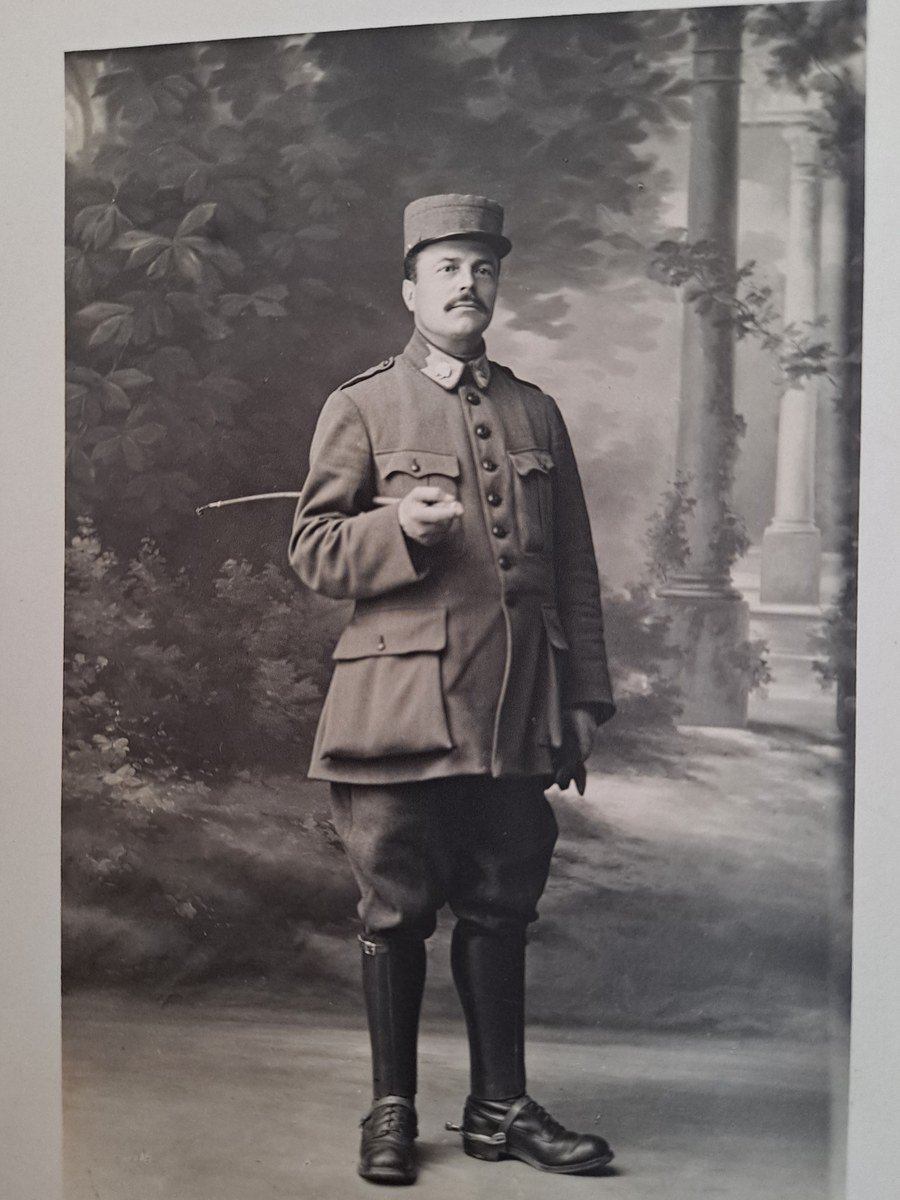
\includegraphics[height=0.34\textheight]{illustrations/hippolyte_interprete_1.jpg}\hspace{4mm}%
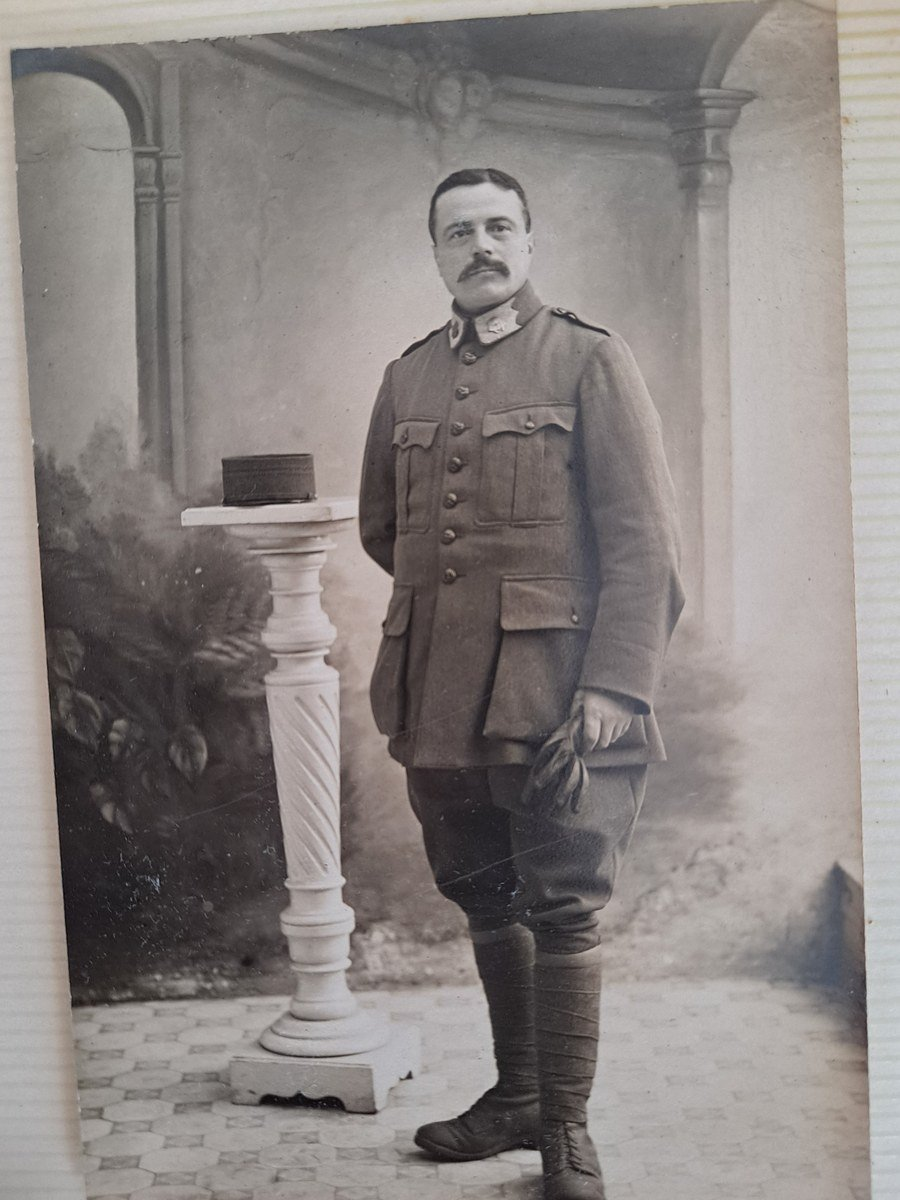
\includegraphics[height=0.34\textheight]{illustrations/hippolyte_interprete_2.jpg}
\caption{Hippolyte Combes en tenue d'interprète, coiffé du képi (à gauche) et tête nue (à droite) ; portraits de studio, 1915--1918 (archives familiales).}\label{fig:interprete}
\end{figure}

\begin{figure}[tbp]
\centering
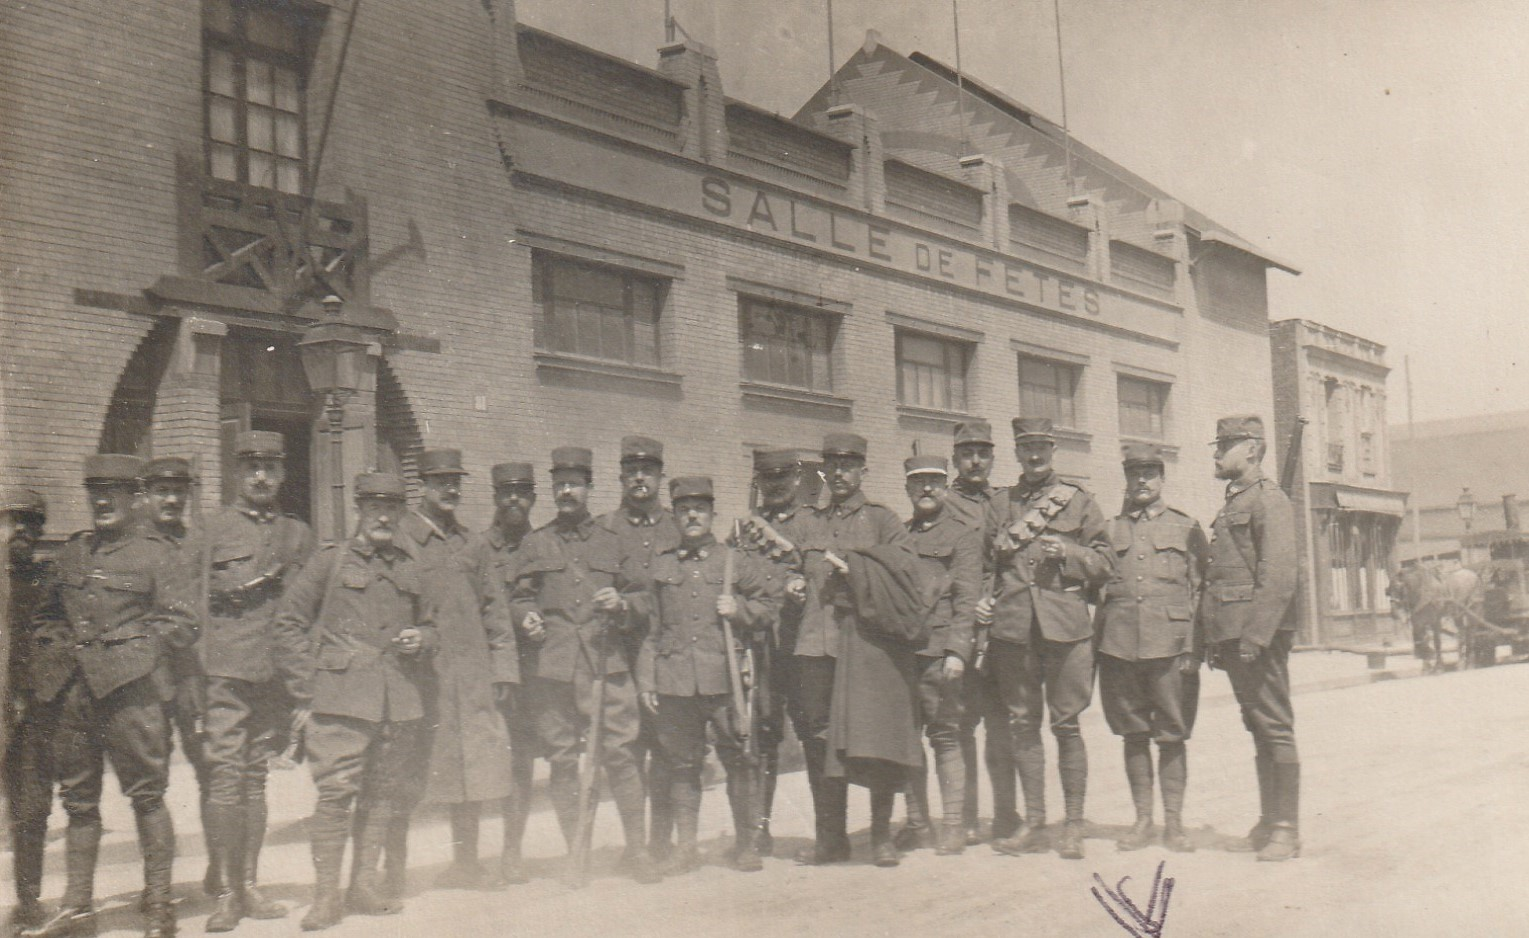
\includegraphics[width=\textwidth,height=0.40\textheight,keepaspectratio]{illustrations/interpretes_salle_des_fetes.jpg}
\caption{Militaires en vareuse kaki de coupe britannique et képi, la tenue des interprètes, devant une salle des fêtes. La famille date cette photographie d'avril 1915, à Toulon, ce que la tenue rend douteux ; ce pourrait être le dépôt des interprètes du Havre, installé à une date inconnue dans «~une petite salle des fêtes~» (Fernand-Laurent, \textit{op.~cit.}, p.~27) ; Hippolyte Combes passa sans doute par Le Havre en mai 1915. Un trait à l'encre, au bas de l'épreuve, désigne peut-être Hippolyte Combes, deuxième à partir de la droite (archives familiales).}
\end{figure}

Hippolyte Combes était auxiliaire.\label{intro:statut} Détaché à la Mission en mai 1915, rattaché pour son administration, à partir du 15~octobre 1915, au 19\textsuperscript{e} escadron du train des équipages militaires, il resta simple soldat jusqu'à sa nomination au grade de caporal, en décembre 1918\footnote{Fiche matricule d'Hippolyte Combes (classe 1896, n\textsuperscript{o}~911), copie numérique, archives familiales. Un détachement du 19\textsuperscript{e} escadron «~administre les secrétaires automobilistes et interprètes~» de la Mission (\textit{19\textsuperscript{e} Escadron du train des équipages militaires. Historique. Guerre 1914--1918}, Paris et Limoges, Charles-Lavauzelle, 1921, p.~49).}. Dans sa lettre de février 1916, il s'informait d'un «~concours pour être nommé stagiaire~», grade qui ouvrait sans doute l'accès au corps des officiers interprètes ; rien n'indique qu'il l'ait passé.

Chaque division britannique avait son bureau de la Mission, dirigé par un officier interprète et tenu par des sous-officiers : à la 18\textsuperscript{th}~Division, le lieutenant Pizzi, dont Hippolyte Combes fait l'éloge dans sa lettre, et les adjudants Lupin (ou Lépin) et Schumacher (f.~12~r\textsuperscript{o}). Corps d'armée et armées avaient les leurs. Ils payaient les interprètes, visaient leurs permissions, décidaient de leurs affectations et recevaient leurs rapports. Devant l'écriteau «~Mission Militaire Française~», raconte un officier britannique, le nouveau venu croyait parfois à une maison de religieux, «~till he has realised that it is the headquarters [\ldots] of the French interpreters attached to the Division~»\footnote{«~Claims~», par «~A Divisional Claims Officer~», \textit{Blackwood's Magazine}, vol.~201, n\textsuperscript{o}~1220, juin 1917, p.~933--941, ici p.~940.}. Le carnet cite les bureaux où Hippolyte Combes se présente : La Croix-du-Bac (f.~5~r\textsuperscript{o}), Roëllecourt (f.~18~v\textsuperscript{o}), Acheux, où la Mission de la division est logée «~dans les parcs du château -- maisonnette toile \& planches~» (f.~22~r\textsuperscript{o}), Bernaville (f.~34~r\textsuperscript{o}), Albert (f.~40~r\textsuperscript{o}).

Détaché à Acheux le 2~novembre 1916, il reste d'abord payé par le bureau divisionnaire d'Albert (ff.~46~r\textsuperscript{o} et 50~r\textsuperscript{o}), puis relève des bureaux de corps et d'armée. Le 5~novembre, il est convoqué au «~bureau mission du corps~» (f.~47~r\textsuperscript{o}), sans doute celui du V~Corps, installé à Acheux depuis le 2~octobre. Le 1\textsuperscript{er}~décembre, deux jours après que le XIII~Corps (lieutenant-général W.~N.~Congreve) a remplacé à Acheux le V (lieutenant-général E.~A.~Fanshawe), il est «~présenté au bureau Mission française XIII\textsuperscript{e} corps et pris en charge~» (f.~52~v\textsuperscript{o}) ; le 13~janvier 1917, au lendemain du retour du V~Corps, il se rend au «~bureau mission V\textsuperscript{e} corps~» (f.~61~v\textsuperscript{o}). Le bureau de corps suivait donc le quartier général\footnote{C.~Baker, \textit{The Long, Long Trail}, notices «~The British V Corps in France and Flanders~» (QG à Acheux le 2~octobre 1916, à Doullens le 29~novembre, de nouveau à Acheux le 12~janvier 1917, à Bihucourt le 2~avril) et «~The British XIII Corps in France and Flanders~» (Acheux le 29~novembre 1916, Doullens le 12~janvier 1917), \url{https://www.longlongtrail.co.uk} (consultées le 18~octobre 2026). La concordance avec le carnet est établie ; le rattachement du bureau au quartier général en est déduit.}. Le 9~février 1917, au bureau de la Mission de la Fifth Army à Toutencourt, il apprend que «~désormais serai administré par l'armée et payé les 3 et 18~de chaque mois~» (f.~75~r\textsuperscript{o}), sans doute parce que son service d'achats dépend de l'armée.

Le bureau est aussi un recours : le 24~décembre 1916, blessé par un propos de son capitaine, il se demande s'il doit y faire rapport (ff.~56~v\textsuperscript{o}--57~r\textsuperscript{o} ; voir p.~\pageref{intro:bloody}). Le bureau décide enfin de son sort. Le 22~octobre, l'adjudant Schumacher lui avait annoncé que «~les 2/3 des interprètes, jeunes R.A.T.~» seraient renvoyés dans les régiments français (f.~42~r\textsuperscript{o}) ; deux jours plus tard, on l'assurait qu'il resterait à la Mission (f.~43~r\textsuperscript{o}) ; le 1\textsuperscript{er}~décembre, il note encore la «~Perspective réintégration prochaine dans régiment d'origine !~» (f.~52~v\textsuperscript{o}). Aucun texte sur cette réduction n'a été retrouvé\footnote{R.A.T. : réserve de l'armée territoriale, où Hippolyte Combes, de la classe 1896, passait sans doute le 1\textsuperscript{er}~novembre 1916 (fiche matricule citée). La mesure serait à chercher dans les dossiers du GQG relatifs aux interprètes (SHD, GR~16~N~509) et dans les listes nominatives de la Mission (GR~17~N~447--448).}.

\subsection{Solde, indemnité et dépenses}

Le carnet note dix-neuf versements de la Mission, du 27~juillet 1916, à Renescure ou à Hazebrouck, au 21~avril 1917, à Toutencourt : 1\,471,05~F en neuf mois\footnote{27~juillet 1916, 84~F (f.~2~r\textsuperscript{o}) ; 4~août, 80,30~F (f.~5~r\textsuperscript{o}) ; 18~août, 84~F (f.~11~r\textsuperscript{o}) ; 5~septembre, 78,75~F (f.~18~v\textsuperscript{o}) ; 21~septembre, 78,75~F (f.~23~v\textsuperscript{o}) ; 8~octobre, 78,75~F (f.~35~r\textsuperscript{o}) ; 18~octobre, 84~F (f.~40~r\textsuperscript{o}) ; 3~novembre, 58,75~F (f.~46~r\textsuperscript{o}) ; 18~novembre, 88~F (f.~50~r\textsuperscript{o}) ; 3~décembre, 78,75~F (f.~53~r\textsuperscript{o}) ; 19~décembre, 84~F (f.~56~r\textsuperscript{o}) ; 5~janvier 1917, 78,75~F (f.~60~r\textsuperscript{o}) ; 19~janvier, 84~F (f.~62~v\textsuperscript{o}) ; 7~février, 78,75~F (f.~74~r\textsuperscript{o}) ; 18~février, 68,25~F (f.~78~r\textsuperscript{o}) ; 3~mars, 43,75~F (f.~81~r\textsuperscript{o}) ; 18~mars, 82~F (f.~85~r\textsuperscript{o}) ; 6~avril, 78,75~F (f.~88~v\textsuperscript{o}) ; 21~avril, 78,75~F (f.~91~r\textsuperscript{o}).}. Ils sont faits par quinzaine, au début et au milieu du mois ; en février 1917, l'armée en fixe les dates aux 3 et 18, que les versements suivants respectent à quelques jours près. Hippolyte Combes nomme parfois les deux éléments de la somme, une fois en toutes lettres : «~Solde \& indemnité de fonctions : 84~francs~» (f.~11~r\textsuperscript{o}). La plupart des montants sont des multiples de 5,25~F : 78,75~F pour quinze jours, 84~F pour seize, 68,25~F pour treize. Chaque jour de permission est retenu à 5~F : «~30~francs retenus pour 6~jours de permission~» en novembre 1916 (f.~46~r\textsuperscript{o}), «~retenue de 35~francs pour 7~jours de permission~» en mars 1917 (f.~81~r\textsuperscript{o}) : la permission réglementaire passe de six à sept jours au 1\textsuperscript{er}~octobre 1916. Le permissionnaire gardant son prêt, la retenue portait sans doute sur la seule indemnité\footnote{«~Les permissions~», \textit{Bulletin des armées de la République}, n\textsuperscript{o}~186, 22~mars 1916, p.~2 (durée «~uniformément de six jours pleins~» ; droit du permissionnaire «~à son prêt pendant tout le temps de son absence~») ; É.~Cronier, \textit{Permissionnaires dans la Grande Guerre}, Paris, Belin, 2013, p.~18 et 32 (sept jours à partir du 1\textsuperscript{er}~octobre 1916 ; cité de seconde main) ; \textit{Bulletin des armées}, n\textsuperscript{o}~268, 17~octobre 1917, p.~2 (sept jours, portés à dix au 1\textsuperscript{er}~octobre 1917).} : probablement une indemnité de 5~F par jour et le prêt du soldat, 0,25~F depuis le 1\textsuperscript{er}~octobre 1915\footnote{«~La nouvelle solde~», \textit{Bulletin des armées de la République}, n\textsuperscript{o}~144, 24--27~octobre 1915, p.~1.}. Aucun règlement retrouvé ne fixe l'indemnité, et plusieurs versements supposent des rappels ou des rajustements que le carnet n'explique pas : 80,30~F, «~y compris 8~francs~» d'un «~supplément~» de juillet (f.~5~r\textsuperscript{o}) ; 58,75~F le 3~novembre 1916, qui ne correspond à aucune quinzaine diminuée des 30~F retenus (f.~46~r\textsuperscript{o}) ; 88~F ; 82~F.

Le revenu mensuel va de 125,75~F (mars 1917) à 164,30~F (août 1916). À 5,25~F par jour, c'est environ le salaire d'un ouvrier des petites industries du Nord (5,63~F en 1916) et une fois et demie celui d'un journalier agricole de la Somme (3,50~F)\footnote{L.~March, \textit{Mouvement des prix et des salaires pendant la guerre}, Paris et New Haven, PUF et Yale University Press, 1925, p.~254 et 264 ; la comparaison est de l'éditeur.} ; mais l'interprète est logé, transporté et en partie équipé par l'armée. Sa plus grosse dépense courante est la table. Le 12~septembre 1916\label{intro:mess}, à la demande insistante du capitaine West, il devient «~membre du mess des officiers à titre définitif~» : «~Cuisine quelconque --- mais grands avantages~» (f.~21~v\textsuperscript{o}). Sa quote-part passe de 29~F en septembre à 47,70~F en octobre, 70~F en novembre (ff.~34~v\textsuperscript{o}, 46~r\textsuperscript{o}, 52~v\textsuperscript{o}), 88~F en décembre (total de sa main, supérieur de 10~F à la somme des montants inscrits) et 79,10~F en janvier (ff.~58~v\textsuperscript{o}, 63~v\textsuperscript{o}) : de novembre à janvier, près de la moitié des versements. Dans une supplique non datée, il plaide pour «~le maintien intégral de notre faible indemnité~», car «~Les Anglais ne sauraient se passer de nous~»\footnote{Minute de lettre à un «~Monsieur le Président~» non identifié, sans date, carnet quadrillé, folio~37, archives familiales (voir l'annexe, doc.~2) ; «~intégral~» et «~faible~» sont des ajouts.}. Il avait peut-être une autre ressource : la loi du 5~août 1914 permettait aux fonctionnaires mobilisés qui n'étaient ni officiers ni sous-officiers à solde mensuelle de cumuler en totalité solde et traitement civil ; on ignore si Hippolyte Combes conserva le sien\footnote{\textit{Larousse mensuel illustré}, n\textsuperscript{o}~109, mars 1916, art. «~Traitement civil~», p.~714--715 ; réponse du ministre de l'Instruction publique à une question écrite du député de Kerguézec, \textit{Les Langues modernes}, 16\textsuperscript{e}~année, 1918, p.~70.}.

\subsection{La 18\textsuperscript{th}~(Eastern) Division et son train}

La 18\textsuperscript{th}~(Eastern) Division appartenait à la deuxième des «~armées nouvelles~» de Kitchener. Autorisée en septembre 1914, formée de bataillons de l'Est-Anglie et des comtés voisins de Londres, rassemblée autour de Colchester, elle débarqua en France à partir du 24~juillet 1915 et se concentra le 30 près de Flesselles.\label{intro:division} Hippolyte Combes lui fut alors attaché ; selon la tradition familiale, il avait d'abord servi auprès du 1\textsuperscript{st}~Battalion, Irish Guards. Le major-général Ivor Maxse, qui l'avait formée, la commanda jusqu'au 15~janvier 1917. Le 25~octobre 1915\label{intro:revue}, sans doute au nord de Ribemont-sur-Ancre, il présenta ses bataillons, avec ceux des 5\textsuperscript{th} et 51\textsuperscript{st}~Divisions, à la revue du roi George~V et du président Raymond Poincaré, en présence du prince de Galles et du général Allenby. Hippolyte Combes y assista et en prit des notes ; c'est très probablement elle que devait raconter le chapitre~\textsc{ix} des \textit{Feuillets de Route}\footnote{A.~F.~Becke, \textit{Order of Battle of Divisions}, part~3A, \textit{New Army Divisions (9--26)}, Londres, HMSO, 1938, p.~79--84 ; G.~H.~F.~Nichols, \textit{The 18\textsuperscript{th}~Division in the Great War}, Édimbourg et Londres, Blackwood, 1922, p.~6 et 22 (Nichols place la revue «~one mile north of Ribecourt~», R.~Poincaré, \textit{Au service de la France}, t.~VII, Paris, Plon, 1931, p.~198, «~à Ribécourt~» : aucune commune du secteur ne porte ce nom ; les notes d'Hippolyte Combes situent le terrain sur la route de Bresle, qui part de Ribemont-sur-Ancre vers le nord) ; pour Flesselles et la revue du 25~octobre 1915, voir l'annexe, p.~\pageref{annexe:doc1-flesselles}, \pageref{annexe:doc6-ix} et~\pageref{annexe:doc7}.}.

Chaque division avait son train (\textit{divisional train}), unité de l'Army Service Corps commandée par un lieutenant-colonel et formée de quatre compagnies hippomobiles : une pour le quartier général et les troupes divisionnaires, une par brigade d'infanterie («~Le ventre d'une brigade~», écrit Hippolyte Combes, \textit{Feuillets de Route}, chap.~\textsc{vii}, annexe, p.~\pageref{annexe:doc6-vii}). Elles portaient vivres, fourrage et bagages de toute la division, sauf le premier échelon des bataillons. Un train comptait à l'origine 26~officiers, 402~hommes, 378~chevaux et 125~voitures\footnote{F.~K.~Puckle, \textit{The Army Service Corps of the British Army and the Organization of the Transport and Transportation at the Front in France}, Washington, Government Printing Office, 1917, p.~8, 10 et 21 ; C.~Baker, \textit{The Long, Long Trail}, «~Army Service Corps Horse Transport Companies~», \url{https://www.longlongtrail.co.uk}.}. Celui de la 18\textsuperscript{th}~Division réunissait les 150\textsuperscript{th}, 151\textsuperscript{st}, 152\textsuperscript{nd} et 153\textsuperscript{rd} Companies, sous les ordres, en 1916, du lieutenant-colonel D.~C.~E.~Grose\footnote{Becke, \textit{op.~cit.}, p.~83, n.~6 ; Nichols, \textit{op.~cit.}, p.~107.}. La 152\textsuperscript{nd}~Company, du capitaine E.~M.~West, servait la 54\textsuperscript{th} Infantry Brigade (11\textsuperscript{th} Royal Fusiliers, 7\textsuperscript{th} Bedfordshire, 6\textsuperscript{th} Northamptonshire, 12\textsuperscript{th} Middlesex) : elle marche dans sa colonne en septembre 1916 et en conduit encore les transports en avril 1917, selon les ordres d'opérations du 7\textsuperscript{th} Bedfordshire\footnote{Journal de marche (\textit{War Diary}) du 7\textsuperscript{th} Bedfordshire, Bedfordshire Archives, X550/8/1/1609, ordres n\textsuperscript{os}~30 et 31 (9 et 10~septembre 1916), et X550/8/1/1704, ordre n\textsuperscript{o}~5 (26~avril 1917) : «~The Transport will proceed by road under Capt. West Comdg 152nd Coy A.S.C.~». Ces documents contemporains contredisent le tableau de Nichols (\textit{op.~cit.}, p.~108--110), qui place la 152\textsuperscript{nd}~Company auprès de la 55\textsuperscript{th}~Brigade.}. Le carnet concorde : il est «~occupé au cantonnement des Royal Fusiliers~», dont il faut loger trente-six officiers (f.~1~v\textsuperscript{o}), attend en vain deux voitures des «~Bedfords~» (f.~19~v\textsuperscript{o}) et, au retour de permission, retrouve sa compagnie au «~refilling point de ma brigade~» (f.~33~v\textsuperscript{o}).

Jusqu'à la fin d'octobre 1916, Hippolyte Combes vit avec la compagnie : il cherche les chambres des officiers et les salles de mess, suit le convoi sur un poney que soigne un \textit{groom}, Connelly, et mène avec le lieutenant Curtis les corvées de fourrage vert (ff.~2~v\textsuperscript{o}, 3~r\textsuperscript{o}, 6~r\textsuperscript{o}, 7~v\textsuperscript{o}). Le 1\textsuperscript{er}~novembre 1916 au soir, Curtis lui apporte l'ordre : «~Nous sommes détachés de la Company Transport~» (f.~45~r\textsuperscript{o}). Le lendemain, au bureau de la Mission, on lui conseille de demander un ordre écrit ; au bureau du train, «~Colonel Grose, signé ordre d'accompagner lieutenant Curtis à Acheux~» (f.~45~v\textsuperscript{o}). \label{intro:detache}«~Regrette d'avoir quitté 152~Company~», écrit-il quatre jours plus tard (f.~47~v\textsuperscript{o}). Il ne revoit le train qu'en passant : un thé au mess de la 152\textsuperscript{nd}~Company le 9~novembre (f.~48~r\textsuperscript{o}), la 150\textsuperscript{th}~Company près d'Hédauville le 9~janvier 1917 (f.~60~v\textsuperscript{o}), «~mon ancienne Company~» sous la tente sur la route d'Aveluy, une semaine avant la bataille de Boom Ravine (f.~75~v\textsuperscript{o}).

\subsection{Ravitailler une armée : du \emph{railhead} au \emph{purchase board}}

\begin{figure}[tbp]
\centering
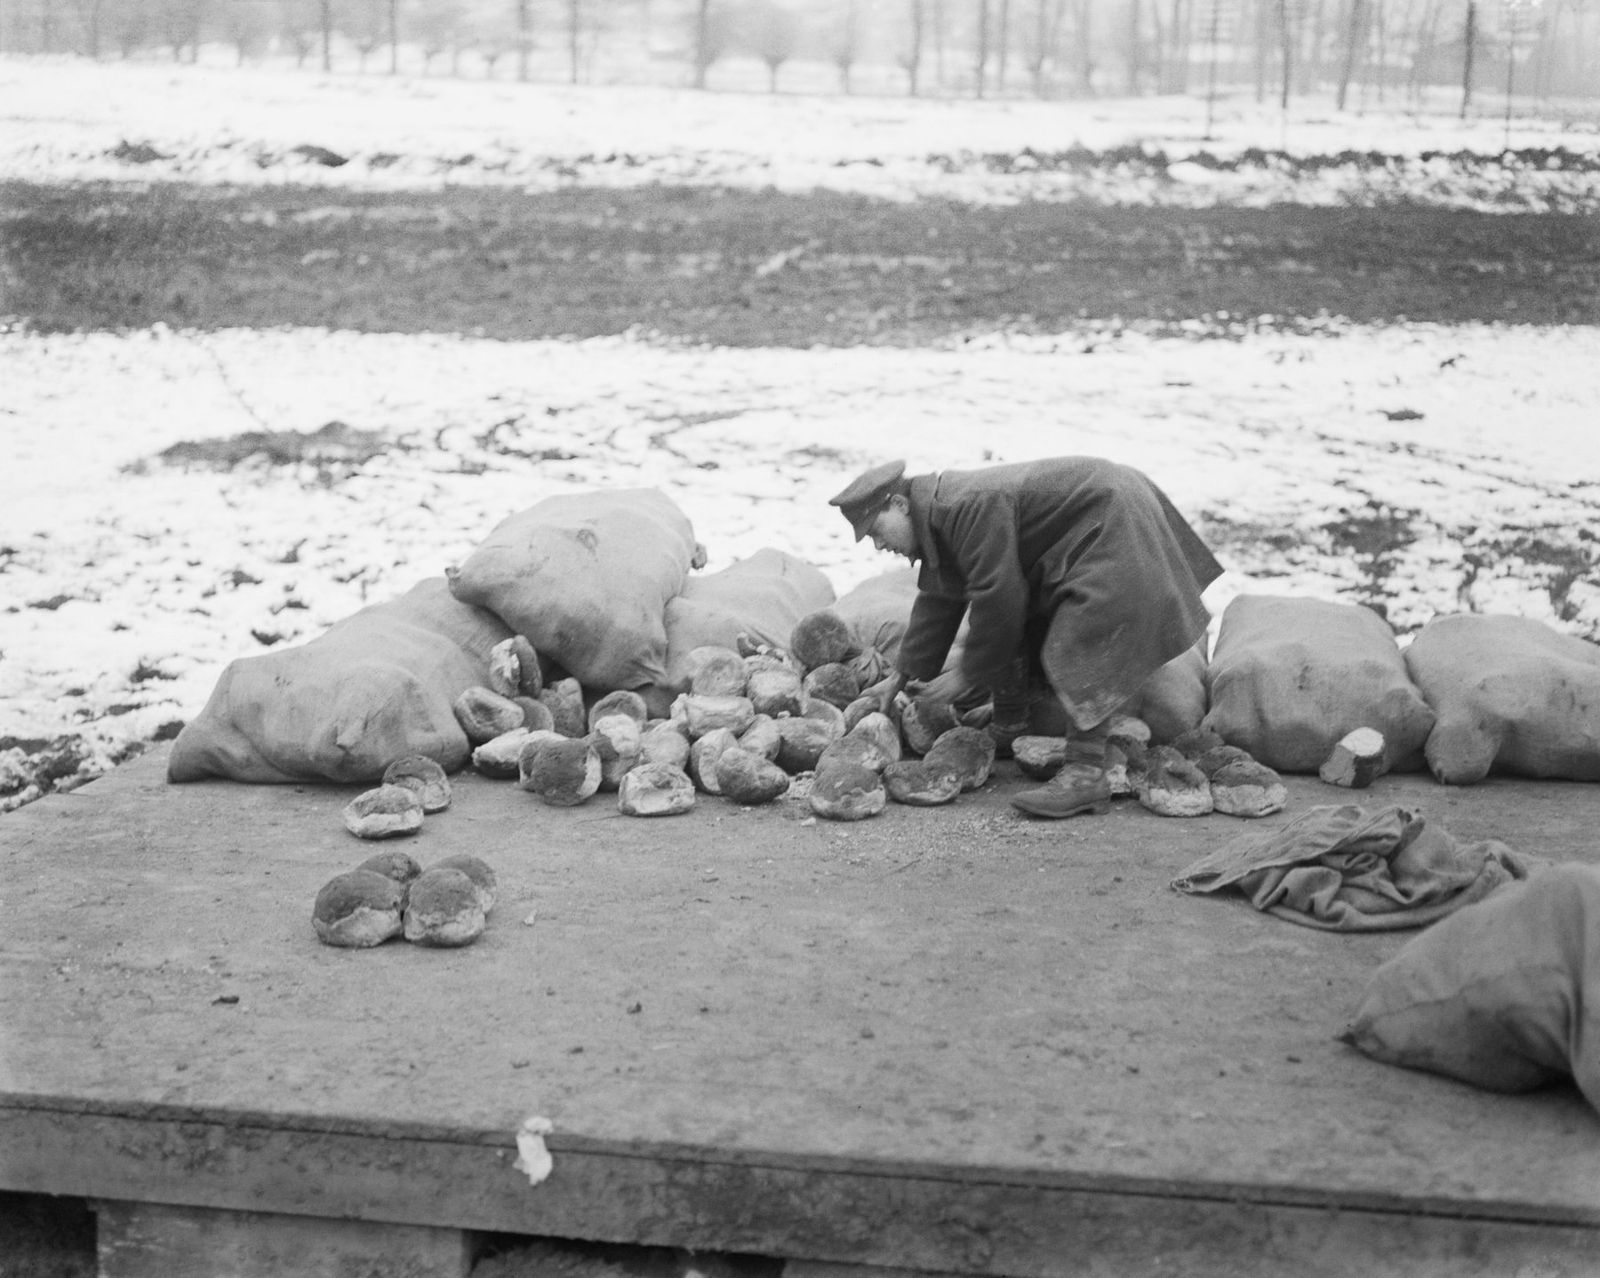
\includegraphics[width=\textwidth,height=0.42\textheight,keepaspectratio]{illustrations/epoque/albert_depot_routier_distribution_pain_mars_1917.jpg}
\caption{Au dépôt routier d'Albert, un homme de l'Army Service Corps fait les parts de pain des unités, mars 1917 (J.~W. Brooke, Imperial War Museums, Q~4828).}
\end{figure}


Vivres et fourrage arrivaient par le rail à une gare de ravitaillement, le \textit{railhead}, situé en 1917 à une distance de trois à dix milles du front. Les camions de l'ASC (\textit{supply column}) les portaient au \textit{refilling point}, où les voitures du train les reprenaient pour les quartiers-maîtres : chargés le lundi, les vivres étaient au \textit{refilling point} le mardi matin et consommés le mercredi\footnote{\textit{Field Service Pocket Book, 1914}, Londres, HMSO, 1914, «~Definitions~» ; Puckle, \textit{op.~cit.}, p.~10--11.}. Ces mots sont familiers au carnet. Le 6~août 1916, Hippolyte Combes va avec Curtis au «~refilling point, sur rive canal~», d'où ils partent «~à la recherche fourrage~» (f.~7~r\textsuperscript{o}). Le 6~octobre, au retour de permission, il apprend que sa division «~a shifté~» et que «~Le railhead est Canaples~» ; il y trouve «~les lorries (supply column) de la 54\textsuperscript{e} brigade~» et monte sur l'un d'eux jusqu'au \textit{refilling point} (f.~33~v\textsuperscript{o}).

Le fourrage pesait lourd. Un cheval de trait lourd du train recevait par jour environ quinze livres d'avoine et deux repas de foin ; l'été, le fourrage vert abondait\footnote{H.~Chesterman, «~With a Train Company in France, 1914--1918~», \textit{The Nineteenth Century and After}, 86, n\textsuperscript{o}~511, septembre 1919, p.~571.} (ray-grass, luzerne, sainfoin, trèfle) et remplaçait parfois une partie de la ration de foin\footnote{\textit{Field Service Pocket Book, 1914}, chap.~6, «~Forage~», §~20 ; L.~J.~Blenkinsop et J.~W.~Rainey (éd.), \textit{Veterinary Services}, Londres, HMSO, 1925, p.~566.}. D'où les corvées de l'été 1916 : faire «~faucher \& peser fourrage~» près de Saint-Jans-Cappel (f.~3~r\textsuperscript{o}), conduire «~un waggon to the fields for green forage~» (f.~3~v\textsuperscript{o}), mener une voiture dans un «~Champ de trèfle rouge~» à Raincheval (f.~22~v\textsuperscript{o}). Ces récoltes étaient payées : l'armée britannique pouvait réquisitionner, comme l'armée française, et les réclamations des habitants passaient par le maire\footnote{«~Claims~», art.~cité, p.~933 et 935--939 ; sur le cantonnement et les indemnités dues à l'habitant, Fernand-Laurent, \textit{op.~cit.}, p.~225--234.}. L'interprète, écrit François de Tessan en 1917, «~sert d'intermédiaire pour les approvisionnements ou les réquisitions de paille et de foin. Il négocie avec les autorités civiles pour le logement des troupes~»\footnote{Préface à Fernand-Laurent, \textit{op.~cit.}, p.~\textsc{xiv}.}.

En novembre 1916, le Shipping Control Board avertit le War Office que la crise du tonnage impose de réduire le fret d'avoine et de fourrage. La ration, déjà diminuée, ne pouvant plus l'être, le War Office propose à Haig de renvoyer en Angleterre une partie de sa cavalerie ou d'acheter davantage sur place. Haig refuse la première solution : dès le 21~novembre, il s'entend avec les Français pour faire hiverner la cavalerie dans l'Orne, où tout son fourrage peut être acheté. De 1914 à 1918, selon l'histoire officielle, on expédia en France un poids d'avoine et de fourrage supérieur à celui des munitions\footnote{W.~Miles, \textit{Military Operations, France and Belgium, 1916}, vol.~II, Londres, Macmillan, 1938 (histoire officielle britannique, ci-après \textit{OH~1916},~II), p.~550 et n.~2.}. Pendant la crise des transports de l'hiver, la ration d'avoine tomba à six livres ; les chevaux des batteries et des colonnes de munitions, devenus bêtes de bât, subirent de très lourdes pertes\footnote{C.~Falls, \textit{Military Operations, France and Belgium, 1917}, vol.~I, Londres, Macmillan, 1940 (ci-après \textit{OH~1917},~I), p.~66.}. Les achats en France relevaient d'un Supplies Purchase Department créé en 1916 et établi à Paris, qui achetait notamment le foin et la paille\footnote{\textit{Statistics of the Military Effort of the British Empire during the Great War, 1914--1920}, Londres, HMSO, 1922, p.~850.}, et, dans chaque armée, d'un \textit{purchase board}. La paille, complément de la ration venue de la base et couchage des troupes, était, selon un officier de l'ASC, «~purchased and handled by an organization in each army called the purchase board~». Le \textit{board} gérait presses et batteuses et pouvait constituer, si le pays le permettait, une réserve d'environ 3\,000~tonnes de paille pressée par armée\footnote{Puckle, \textit{op.~cit.}, p.~28.}.

Hippolyte Combes passe dans ce service les six derniers mois du carnet. Le 29~octobre 1916, il enquête déjà à Acheux et à Senlis «~au sujet de straw \& hay disponibles~» (f.~44~r\textsuperscript{o}). Le 2~novembre au soir, à peine arrivé à Acheux, il voit à Raincheval le major Levy, «~of the D.O.S.T.~» (f.~46~r\textsuperscript{o}), qui semble diriger l'«~Army Purchase Board~» installé dans ce village (f.~56~r\textsuperscript{o})\footnote{«~D.O.S.T.~» : lecture assurée ; peut-être l'abréviation britannique \textit{D. of S. and T.}, \textit{Director of Supplies and Transport} (Puckle, \textit{op.~cit.}, p.~26), ou une mauvaise audition de \textit{D.D.S.T.}, \textit{Deputy Director of Supplies and Transport}, chef de l'ASC à l'échelon de l'armée (\textit{ibid.}, p.~8). Le major Levy n'est pas identifié avec certitude : le seul major de l'ASC de ce nom relevé dans la \textit{London Gazette} est Walter Henry Levy, major temporaire au 1\textsuperscript{er}~mai 1916 (\textit{Supplement to the London Gazette}, n\textsuperscript{o}~29585, 17~mai 1916, p.~4941), qu'aucune source consultée ne place à la tête d'un \textit{purchase board}.}. Avec le lieutenant Curtis, puis, à partir du 2~décembre, le capitaine Williams, âgé de vingt ans (f.~53~v\textsuperscript{o}), il parcourt en automobile les villages entre l'Authie et l'Hallue : achat de paille et de foin à Coisy (f.~47~v\textsuperscript{o}), battage à Arquèves (f.~54~r\textsuperscript{o}), location d'une machine à battre à Beauquesne (ff.~57~v\textsuperscript{o} et 60~r\textsuperscript{o}), «~expertise machine endommagée~» dans une ferme de Louvencourt (f.~59~r\textsuperscript{o}), réunion des réfugiés d'Englebelmer à la mairie de Toutencourt en présence du major Levy (f.~55~r\textsuperscript{o}), visites aux maires et au notaire (ff.~59~v\textsuperscript{o}, 87~v\textsuperscript{o}). Le 7~février 1917, au retour de permission, il trouve le bureau à Hérissart, transféré à trois kilomètres du quartier général de la Fifth Army (ff.~73~v\textsuperscript{o}--74~r\textsuperscript{o}). Les tournées «~de ferme en ferme pour trouver paille \& foin~» (f.~78~v\textsuperscript{o}) durent jusque sous la neige d'avril (f.~88~r\textsuperscript{o}). La Mission lui a prescrit de rester auprès du capitaine Williams jusqu'à son départ, «~puis me rendre au dépôt, Toutencourt~» (f.~82~r\textsuperscript{o}) ; ce départ, le 10~mars, le laisse «~sans fonctions~» (f.~82~v\textsuperscript{o}). Le lendemain, il dépose ses sacs «~au mess des interprètes~», mais apprend au bureau que, «~sur demande instante du major Levy~», il restera «~au Purchase Board~» (f.~83~r\textsuperscript{o}). Le 21~avril, il note : «~Cherché vainement paille à acheter~» (f.~91~r\textsuperscript{o}).

\subsection{Le cadre militaire, de la Lys à l'Ancre}

\begin{figure}[tbp]
\centering
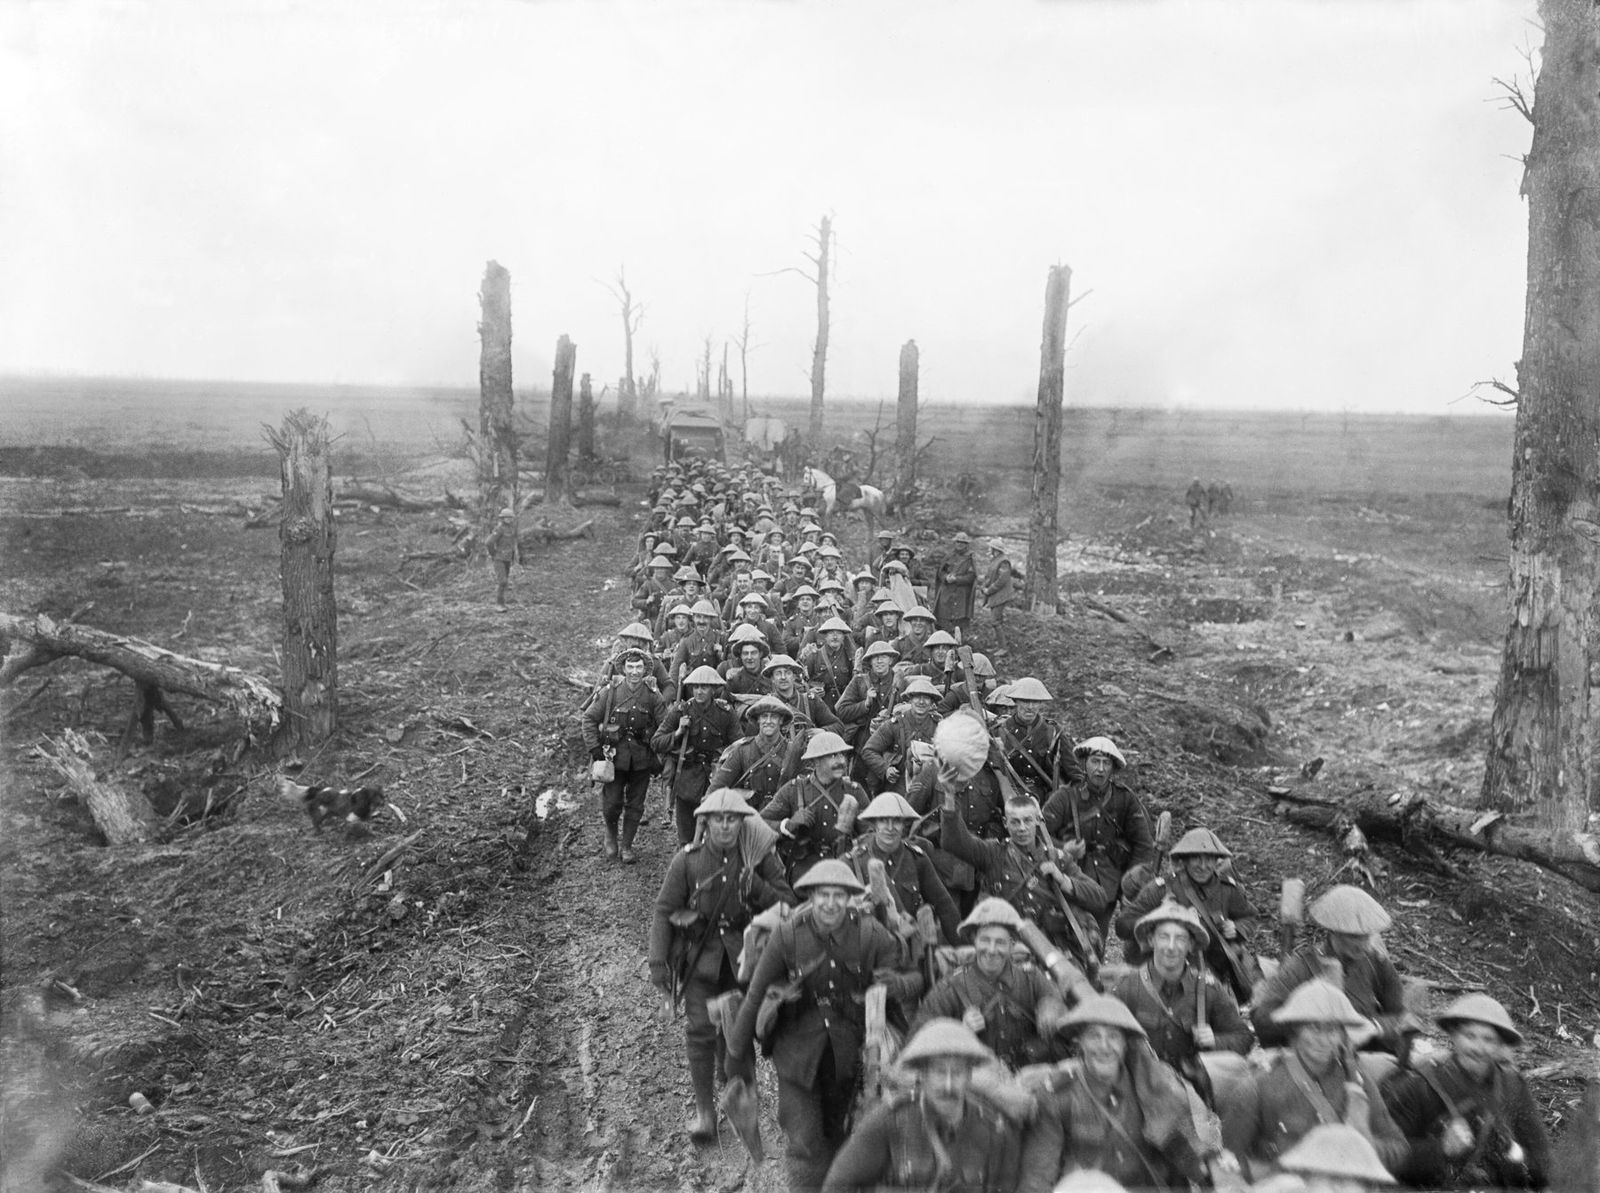
\includegraphics[width=\textwidth,height=0.42\textheight,keepaspectratio]{illustrations/epoque/repli_allemand_route_amiens_saint_quentin_mars_1917.jpg}
\caption{Mars 1917, le repli allemand sur la ligne Hindenburg : l'infanterie britannique avance sur la route d'Amiens à Saint-Quentin (E.~Brooks, Imperial War Museums, Q~1863).}
\end{figure}


En juillet 1916, la 18\textsuperscript{th}~Division sort de la bataille de la Somme, livrée dans le XIII~Corps de la Fourth Army : à Montauban le 1\textsuperscript{er}~juillet, puis au bois des Trônes et au bois Delville du 14 au 21~juillet\footnote{Becke, \textit{op.~cit.}, p.~84 ; Nichols, \textit{op.~cit.}, p.~51--74.}. Transportée en Flandre, elle passe à la Second Army du général Plumer (front de Laventie à Boesinghe). Sa 54\textsuperscript{th}~Brigade se repose autour de Wallon-Cappel, gagne le 28~juillet les environs de Bailleul et relève, dans la nuit du 6 au 7~août, des Néo-Zélandais au sud-est d'Armentières, «~astride the Armentières-Lille road~», tandis que la compagnie d'Hippolyte Combes cantonne à La Croix-du-Bac (f.~6~r\textsuperscript{o})\footnote{Journal de marche du 7\textsuperscript{th} Bedfordshire, X550/8/1/1607--1608 (juillet--août 1916) ; \textit{OH~1916},~II, p.~543, n.~3.}. Son corps d'armée était probablement le II ANZAC Corps, qui tenait le secteur depuis juillet\footnote{\textit{OH~1916},~II, p.~121, n.~1.}. Le secteur est calme\footnote{Nichols, \textit{op.~cit.}, p.~75 : «~August was spent in a quiet part of the line in front of Armentières, and there was intensive training~».}, mais le 11~août «~40 ou 50~obus~» tombent «~autour de nos parages~» (f.~9~r\textsuperscript{o}).

Les 24 et 25~août, la brigade est transportée de Bailleul à Saint-Pol : trois semaines d'instruction dans la zone de la Third Army, autour de Marquay et de La Thieuloye (attaque sous bois, attaque à l'aube, progression derrière un barrage). Un premier ordre de transfert à la Reserve Army, pour la nuit du 6 au 7~septembre, est annulé le 5 au matin, d'où la plainte du carnet ce jour-là : «~encore 8~jours à moisir ici, hélas !~» (f.~18~v\textsuperscript{o}). Le transfert prend effet dans la nuit du 10 au 11~septembre, à minuit ; la brigade gagne Raincheval en trois étapes\footnote{Journal de marche du 7\textsuperscript{th} Bedfordshire, X550/8/1/1608--1609, notamment les ordres n\textsuperscript{os}~28 (4~septembre, annoté «~Cancelled 5 a.m. 5.9.16~») et 29 (8~septembre). Nichols (\textit{op.~cit.}, p.~78) date du 8~septembre le rattachement au II~Corps.}.

La division passe alors au II~Corps du lieutenant-général C.~W.~Jacob, dans la Reserve Army du général Gough, qui devient la Fifth Army le 30~octobre 1916\footnote{Becke, \textit{op.~cit.}, p.~84 ; Baker, \textit{The Long, Long Trail}, «~The British Fifth or Reserve Army 1916--1918~» ; \textit{OH~1916},~II, p.~460, n.~1, qui écrit seulement «~at the end of October~».}. Pendant la permission d'Hippolyte Combes, elle prend Thiepval (26--27~septembre) et dispute la Schwaben Redoubt jusqu'au 5~octobre ; après un repos vers Candas, elle revient devant l'Ancre. Le 21~octobre, sa 53\textsuperscript{rd}~Brigade prend Regina Trench. Le 18~novembre, sa 55\textsuperscript{th}~Brigade attaque Desire Trench, dernier épisode de la bataille de l'Ancre (13--18~novembre), date que l'histoire officielle retient pour la fin des batailles de la Somme\footnote{\textit{OH~1916},~II, p.~\textsc{xliv}, 463 et 514--517 ; Nichols, \textit{op.~cit.}, p.~79--82, 126 et 130--136.}. Hippolyte Combes entend ces combats : d'Albert, le 20~octobre, un «~Duel d'artillerie formidable~» (f.~41~r\textsuperscript{o}) ; d'Acheux, où il voit passer les blessés le 14~novembre (f.~49~r\textsuperscript{o}), une «~très violente canonnade vers Beaumont sur Ancre~» le lendemain (f.~49~v\textsuperscript{o}).

Relevée fin novembre, reposée vers Abbeville, la division revient sur l'Ancre le 16~janvier 1917, quand le II~Corps relève le IV~Corps au sud de la rivière\footnote{Nichols, \textit{op.~cit.}, p.~136 et 139 ; \textit{OH~1917},~I, p.~69.}. Hippolyte Combes, lui, reste à Acheux, où le V~Corps, revenu le 12~janvier, reprend le secteur du XIII, au nord de l'Ancre\footnote{Baker, notices citées ; \textit{OH~1917},~I, p.~66 et 69.}. Le 10~février, il passe au bureau de la Mission du II~Corps, revenu à Senlis le 21~janvier (f.~75~v\textsuperscript{o})\footnote{Baker, \textit{The Long, Long Trail}, «~The British II Corps in France and Flanders~» (QG à Senlis du 24~juillet au 1\textsuperscript{er}~décembre 1916, puis à partir du 21~janvier 1917).}. Le 17~février, au début du dégel, la division attaque à Boom Ravine, près de Miraumont, dans une boue profonde ; elle y perd 54~officiers et 1\,135~hommes\footnote{\textit{OH~1917},~I, p.~75--82 ; Nichols, \textit{op.~cit.}, p.~139--143.}.

Les Allemands commencent alors à se replier : le 24~février, des patrouilles de la 18\textsuperscript{th}~Division trouvent leurs lignes avancées évacuées ; le repli général sur la ligne Hindenburg, préparé par le plan Alberich, s'achève le 19~mars. La division prend Irles le 10~mars, poursuit l'ennemi jusqu'à Saint-Léger, est relevée le 20 et quitte la Somme du 22 au 27~mars pour un mois de repos entre Aire et Hazebrouck ; elle sera engagée le 3~mai devant Chérisy, dans le VII~Corps de la Third Army\footnote{\textit{OH~1917},~I, p.~95--101, 110--115 et 143--145 ; Nichols, \textit{op.~cit.}, p.~155--166 ; Becke, \textit{op.~cit.}, p.~85.}. De la cavalerie indienne traverse Hérissart le 28~février (f.~80~r\textsuperscript{o}), de la cavalerie «~indigène \& anglaise~» le 17~mars (f.~84~v\textsuperscript{o}) ; le 21, près de Senlis, Hippolyte Combes admire les «~Death or Glory Boys, 17\textsuperscript{th} Lancers~» (f.~85~v\textsuperscript{o}), régiment de la 4\textsuperscript{th} Cavalry Division, alors engagée dans la poursuite\footnote{Baker, \textit{The Long, Long Trail}, «~1\textsuperscript{st} Indian Cavalry Division (later 4\textsuperscript{th} Cavalry Division)~» (4\textsuperscript{th} Cavalry Division à partir de novembre 1916) ; \textit{OH~1917},~I, p.~138, 140 et 368.}. L'arrière-front se vide : le quartier général de la Fifth Army quitte Toutencourt pour Albert le 28~mars, celui du V~Corps quitte Acheux le 2~avril\footnote{Baker, notices citées.}. À Hérissart, «~Village paraît abandonné. Plus de troupes.~» (f.~87~r\textsuperscript{o}) ; Toutencourt est «~si tranquille, depuis départ H.Q. et troupes~» (f.~88~v\textsuperscript{o}). Le 9~avril s'ouvre la bataille d'Arras : assaut des Third et First Armies, prise de la crête de Vimy par le corps canadien, attaque de la Fifth Army à Bullecourt le 11, deuxième bataille de la Scarpe les 23 et 24~avril\footnote{\textit{OH~1917},~I, chap.~\textsc{viii}--\textsc{xv}.}. D'Hérissart, à une quarantaine de kilomètres, Hippolyte Combes entend dans la nuit du 20 au 21~avril une «~violente canonnade --- sud d'Arras~» (f.~91~r\textsuperscript{o}).

\subsection{La météorologie du carnet}

Les notations météorologiques, presque quotidiennes, concordent avec l'histoire officielle, ce qui conforte la confiance dans ses autres observations datées. L'orage et la «~pluie torrentielle~» de la nuit du 18 au 19~octobre 1916 (f.~40~v\textsuperscript{o}) précèdent l'ajournement, annoncé le 19 au matin, de l'attaque de Regina Trench, livrée le 21 par un temps que l'histoire officielle dit beau et froid ; le carnet note ce jour-là : «~Nuit très froide. Gelé fortement~» (f.~41~v\textsuperscript{o}). La pluie reprend le 24 (f.~43~r\textsuperscript{o}). L'assaut de Desire Trench part dans la «~première neige~» du 18~novembre (f.~50~r\textsuperscript{o}). Le 14~janvier 1917, quand le gel raffermit enfin le terrain selon l'histoire officielle, il neige «~à gros flocons~» (f.~61~v\textsuperscript{o}) ; le 16, Hippolyte Combes note : «~Nuit, gelé très fort~» (f.~62~r\textsuperscript{o}). Le froid dure un mois. Le 25, par 15~°F (−9,4~°C), il écrit «~gelé extrêmement + fort~», après avoir trouvé la veille l'eau gelée dans son pot et son seau (f.~63~v\textsuperscript{o}). Le 8~février, la «~Terre durcie jusqu'à grande profondeur~» (f.~74~v\textsuperscript{o}) répond au sol gelé en profondeur de la dépêche de Haig, et le «~dégel très rapide~» du 16~février (f.~77~v\textsuperscript{o}) à celui de l'histoire officielle. Concordent aussi la neige de la nuit du 4 au 5~mars, la «~tourmente de neige~» du 4~avril, le beau temps de Pâques, la grêle, le grésil et la neige des 9, 10 et 11~avril, pendant l'offensive d'Arras (ff.~81~r\textsuperscript{o}, 88~r\textsuperscript{o}, 89~r\textsuperscript{o}--v\textsuperscript{o})\footnote{\textit{OH~1916},~II, p.~461--462 et 514 ; \textit{OH~1917},~I, p.~66, 69, 76, 104, 159, 161, 168, 201 et 364 ; J.~H.~Boraston (éd.), \textit{Sir Douglas Haig's Despatches (December 1915 -- April 1919)}, Londres, Dent, 1919, p.~69--70. Même concordance pour l'été 1916 dans le journal de marche du 7\textsuperscript{th} Bedfordshire : «~A very hot day which tired the men severely~», le 28~juillet ; «~chaleur intense~», écrit Hippolyte Combes le même jour (f.~2~v\textsuperscript{o}).}.
